% Manuscript source. Article class, natbib, note-free bibliography (built by build.sh),
% SVG figures converted to PDF by build.sh. Every stated number traces to a committed
% run record; the anchor is results/benchmark/benchmark_r1-union.json (see REPRODUCE.md).
\documentclass[11pt]{article}

\usepackage[T1]{fontenc}
\usepackage[utf8]{inputenc}
\usepackage{lmodern}
\usepackage[margin=1in]{geometry}
\usepackage{booktabs}
\usepackage{multirow}
\usepackage{graphicx}
\usepackage{xcolor}
\usepackage{amsmath}
\usepackage{amssymb}
\usepackage[numbers,sort&compress]{natbib}
\usepackage{hyperref}
\hypersetup{colorlinks=true, allcolors=blue}

\title{How Much Does Physics Buy You?\\ A Physics-Informed vs Black-Box Benchmark for Greenhouse Climate Control\thanks{Preprint. All numbers trace to the committed run records in release v1.0.0 of the code repository; the reproducibility statement gives the anchor and command map.}}
\author{Mohsen Davarynejad, Ph.D.$^{1,2}$ \\ \small $^{1}$Growmatics B.V., \url{https://growmatics.ai} \\ \small $^{2}$Breda University of Applied Sciences (BUas) \\ \small The author is affiliated with both institutions. Corresponding author: \href{mailto:mohsen@growmatics.ai}{mohsen@growmatics.ai} \\ \small ORCID: \href{https://orcid.org/0000-0002-5376-3680}{0000-0002-5376-3680}}
\date{Draft, July 2026}

\begin{document}
\maketitle

\begin{abstract}
Learned controllers promise better economics for greenhouse climate control, but the interaction data they need is the practical obstacle: every training sample on a real greenhouse costs energy, crop risk, and time. Physics-based controllers need no training data but inherit the errors of their model. This paper measures that trade directly. On GreenLight-Gym2, a validated open greenhouse simulator, we benchmark the physics-to-learning spectrum: the rule-based incumbent, black-box reinforcement learning (on-policy PPO and off-policy SAC), physics-only economic nonlinear MPC, and a physics-informed RL-in-MPC hybrid. All run through one harness on an identical grid: four held-out weather years, a controller-model mismatch ladder ($0\%$ to $20\%$, six levels), and five seeds, scored on net economic value, a season-level humidity feasibility gate, online decision cost, and solver reliability. Black-box PPO trained with the simulator's reference recipe reaches $+3.50$~EUR\,m$^{-2}$ held-out net value at 2M environment steps (seed-level SD $0.24$ over five seeds), crossing break-even between 400k and 1M steps, while the myopic economic NMPC ($-3.06 \pm 0.90$) does not outperform the rule-based incumbent ($-2.74 \pm 5.41$). On this deterministic, single-crop, fixed-price testbed the pragmatic winner is black-box RL: it matches the physics-informed RL-in-MPC hybrid on net value at two orders of magnitude lower online cost and with lower humidity degree-hours. The hybrid's only measured advantage is insensitivity to controller-model parameter error (near-flat net value across the mismatch ladder, widening the physics-arm gap to ${\approx}+10$~EUR\,m$^{-2}$ at $20\%$ mismatch, where pure NMPC decays steeply); the effect is large and statistically significant on the six-level ladder ($p < 10^{-12}$), and it is carried by the hybrid's model-free guide, which by construction ignores the perturbed model, not by the physics. The learned policies show no generalization gap (train-year and held-out net agree within year variance). Every controller violates the humidity bound in every season under the native economic objective, confirming that constraint satisfaction must be gated rather than priced. Physics buys instant, training-free competence, but on this testbed the learned controller overtakes it within roughly 55 simulated seasons of experience. Code, run records, and the benchmark protocol are released for reuse.
\end{abstract}

\vspace{0.4em}
\noindent\textbf{Keywords:} greenhouse climate control; model predictive control; reinforcement learning; physics-informed control; benchmarking; data efficiency; constrained control; controlled-environment agriculture.

\section{Introduction}\label{sec:intro}

Greenhouse climate control couples a fast, actuated climate loop to slow crop growth \citep{vanhenten2009timescale, vanstraten2010survey}, under hard biological limits and energy-dominated costs \citep{stanghellini1987transpiration, vanbeveren2015optimal}. The field's methods span a spectrum: rule-based setpoint schedules deployed in practice, economic model predictive control built on greenhouse physics, and reinforcement learning trained on simulated experience \citep{vanlaatum2024greenlight, vanlaatum2026rlmpc}. What is missing is a controlled measurement of the trade that separates them: \emph{how much training data does learning need to match or beat what physics provides for free, and does the physics advantage survive an imperfect model?}

This paper instantiates the evaluation agenda of its companion survey as a concrete, reproducible benchmark. The contribution is the controlled comparison across the physics-to-learning spectrum, not any individual controller: each arm is a faithful implementation of published practice, run on identical conditions with pre-registered metrics.

\section{Related work}\label{sec:related}

\paragraph{Prior work on the substrate.} GreenLight-Gym validates the GreenLight greenhouse model as an RL benchmark and ships PPO/SAC baselines against a rule-based controller under parametric uncertainty \citep{vanlaatum2024greenlight}. Its authors then moved toward hybrids: injecting RL rollouts into a short-horizon economic MPC \citep{vanlaatum2026rlmpc}, and learning terminal ingredients inside stochastic MPC (RL-SMPC) \citep{vanlaatum2026rlsmpc}. Our arm 4 deliberately \emph{reuses} the first of these, reimplemented from the paper; the contribution here is not a new controller but the controlled cross-class, budget-swept, mismatch-swept comparison that no work on this substrate has run. Beyond that group, learned dynamics inside predictive control have been applied to lettuce climate \citep{soumo2025bilstm}, and an independent group learns the MPC parametrization online by Q-learning on a separate greenhouse model \citep{mallick2025rlmpc}; no multi-controller benchmark by a group other than the environment's authors has been reported on GreenLight-Gym itself.

\paragraph{Benchmark-suite precedents.} safe-control-gym is the structural precedent: one suite comparing performance, data efficiency, and safety across classical, learning-based, and RL control on cart-pole and quadrotors, finding model-based control orders of magnitude more data-efficient than model-free RL \citep{yuan2022safecontrolgym}. Safety Gym established constraint-violation rate as a first-class benchmark metric \citep{ray2019safetygym}, and PILCO anchors the data-efficiency framing historically \citep{deisenroth2011pilco}. Our novelty relative to this line is the domain and its consequences: seasonal episodes with economic objectives, held-out weather years, a crop-safety gate, and a controller-model mismatch axis absent from those suites. The guarantee/assumption ledger we report (Table~\ref{tab:ledger}) is grounded in the constrained- and economic-MPC canon \citep{mayne2000constrained, angeli2012economicmpc} and the safe-learning line of control-barrier functions and predictive safety filters \citep{ames2019cbf, wabersich2021safetyfilter}; the benchmark measures where each controller class sits against those guarantees rather than proposing new theory.

\paragraph{Surveys and the field's claim.} Physics-informed reinforcement learning and safe physics-informed machine learning are mapped by method-general surveys \citep{banerjee2025pirl, drgona2025safepiml, nghiem2023pimlcontrol}, learning-based MPC by \citet{hewing2020lbmpc}, and greenhouse control from the classical optimal-control lineage \citep{vanstraten2010survey} to recent strategy reviews \citep{greenhouse_control_review_2025, goldenits2024rldt}; the hybrid-modelling argument itself goes back to \citet{karniadakis2021physics}. These works repeat the claim this paper measures: that physics reduces the data a learned controller needs. The companion survey (in preparation) specifies the evaluation agenda this benchmark instantiates.

\section{Benchmark design}\label{sec:design}

Figure~\ref{fig:setup} summarises the design; Figure~\ref{fig:arch} details the four controller architectures and where physics enters each. The five arms span these four classes: the black-box class holds two learners, on-policy PPO and off-policy SAC, the latter included to test whether the data-efficiency result is specific to PPO.

\begin{figure}[t]
  \centering
  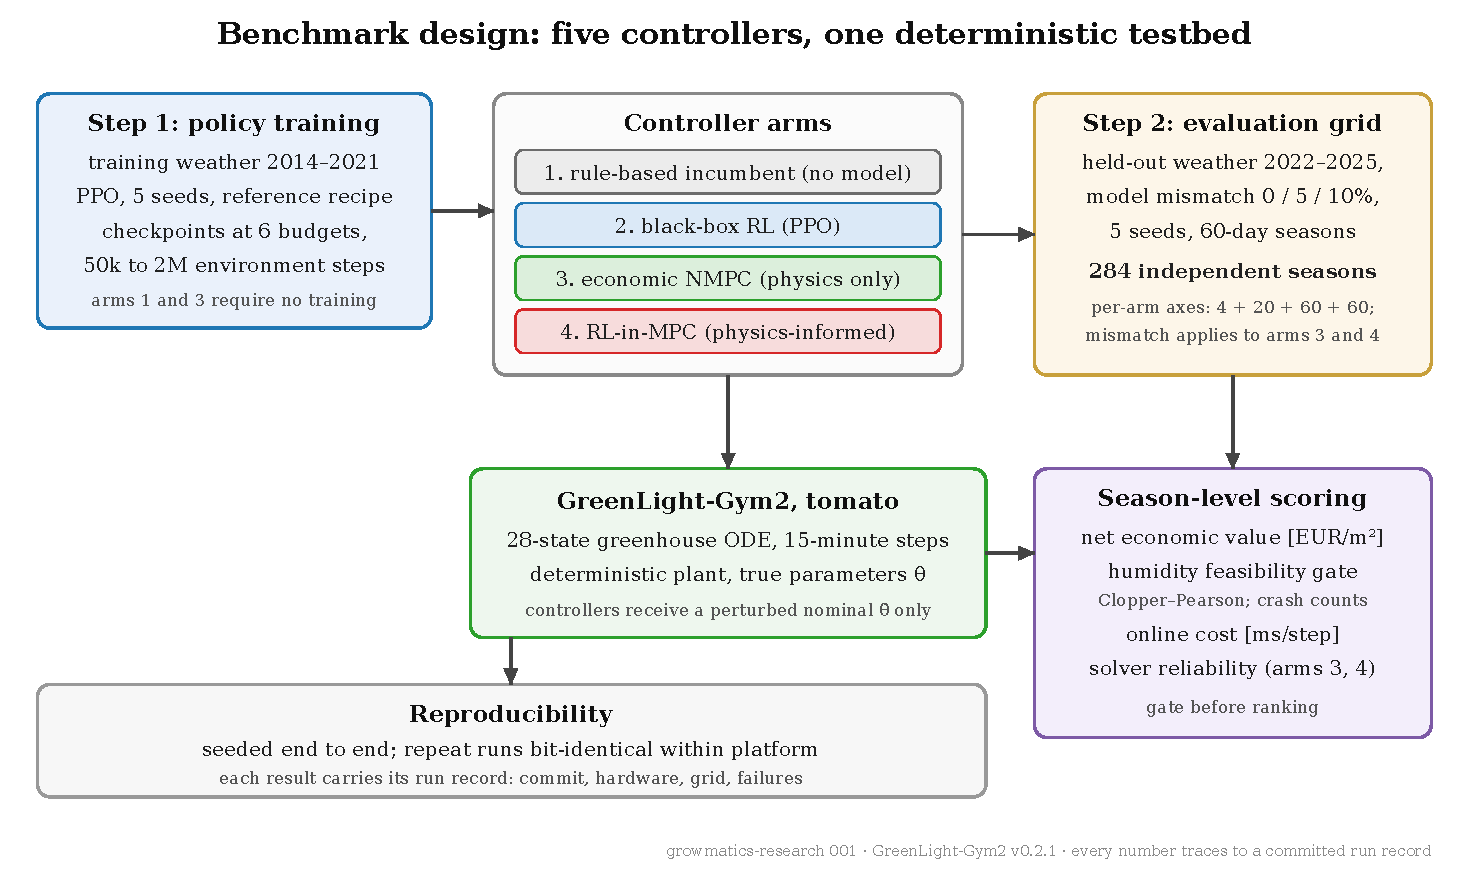
\includegraphics[width=\linewidth]{fig-experimental-setup.pdf}
  \caption{The two-step benchmark. Only the learning arms need training (step~1); all five arms sit the same 284-season exam (step~2). Controllers receive a perturbed nominal model $\tilde\theta$, never the plant's true parameters $\theta$; the mismatch axis perturbs $\tilde\theta$ only. Every number traces to a committed run record.}
  \label{fig:setup}
\end{figure}

\begin{figure}[t]
  \centering
  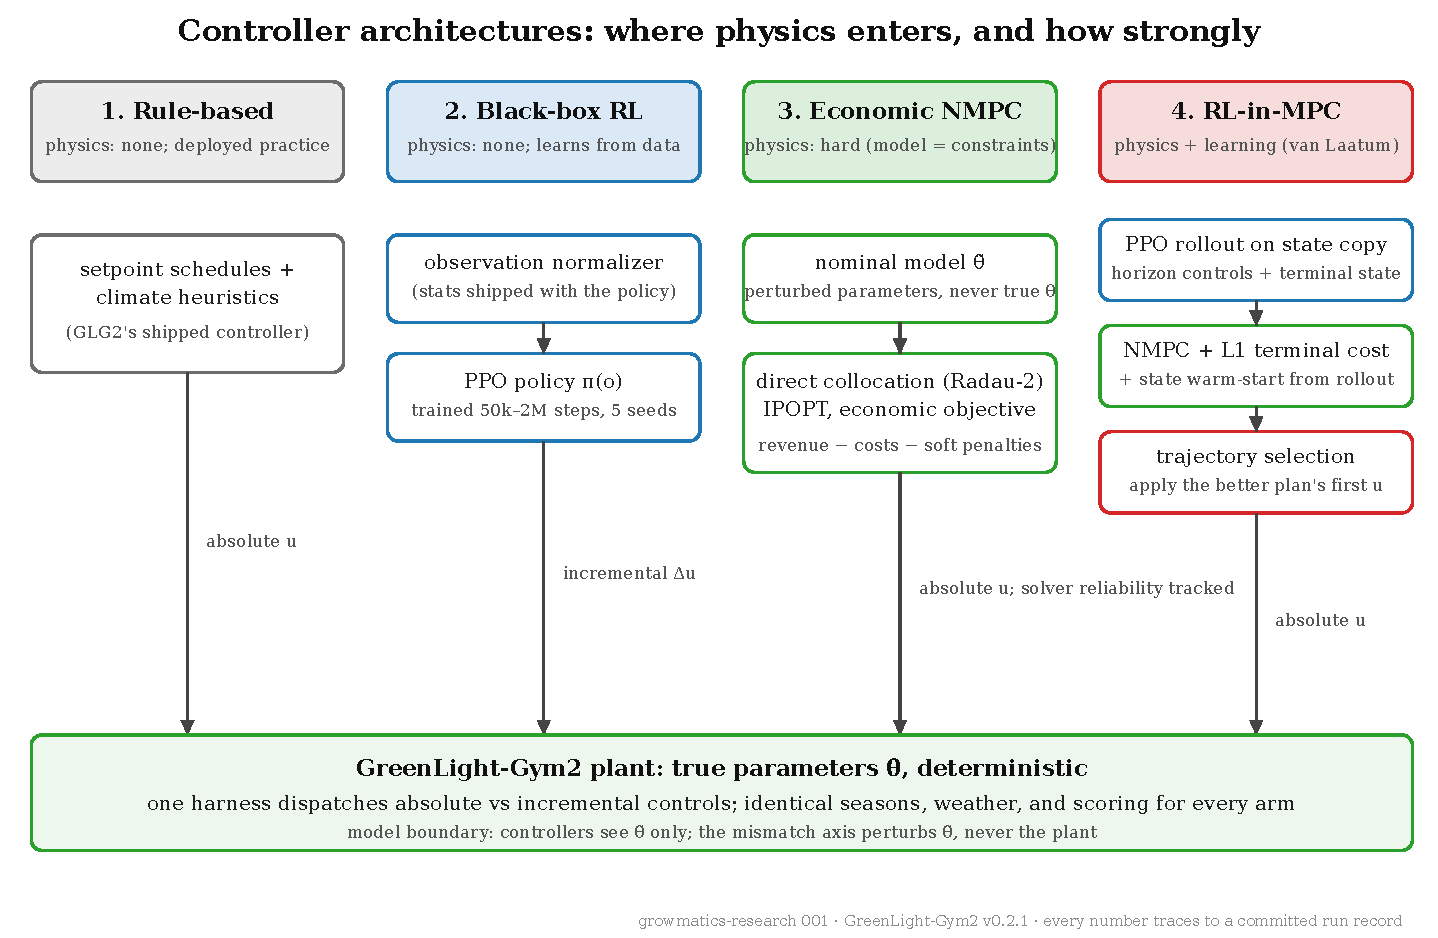
\includegraphics[width=\linewidth]{fig-system-architecture.pdf}
  \caption{The four controller classes ordered by how physics enters: none (rules), none-pays-with-data (PPO with its shipped observation normaliser), hard physics (economic NMPC by direct collocation on the nominal model), and the hybrid (PPO rollout supplies a terminal target and state warm-start to the NMPC; a trajectory-selection step applies the better plan). A second black-box learner, SAC, shares the PPO arm's architecture and is not drawn separately.}
  \label{fig:arch}
\end{figure}

\paragraph{Testbed.} GreenLight-Gym2 \citep{vanlaatum2024greenlight}, tomato crop: a 28-state stiff greenhouse ODE at 15-minute control steps, deterministic given (weather, seed). Weather is real Amsterdam data; training years 2014--2021, held-out years 2022--2025; 60-day seasons.

\paragraph{Problem formulation.} The plant is a deterministic stiff ODE
$\dot{x} = f(x, u, d; \theta)$ with state $x \in \mathbb{R}^{28}$, controls
$u \in [0,1]^{6}$, exogenous weather $d$, and true parameters $\theta$, discretised at
$\Delta t = 15$ min over a season of $T = 5760$ steps, integrated by CVODES
\citep{hindmarsh2005sundials}. A controller receives only a perturbed nominal model
$\tilde\theta_i = \theta_i (1 + \delta_i)$, $\delta_i \sim \mathcal{U}(-m, m)$, at
mismatch level $m \in \{0, 0.025, 0.05, 0.10, 0.15, 0.20\}$; the plant always runs $\theta$. The season
score is the net economic value
\begin{equation}
  J \;=\; \sum_{t=1}^{T} \Big( p_{\mathrm{fruit}}\, \Delta y_t
  \;-\; c_{\mathrm{heat}}\, q_t \;-\; c_{\mathrm{elec}}\, e_t
  \;-\; c_{\mathrm{CO_2}}\, \phi_t \Big),
  \label{eq:epi}
\end{equation}
with fruit growth $\Delta y_t$ and resource flows $(q_t, e_t, \phi_t)$ priced by the
testbed's economic parameters; constraint violations are deliberately absent from
Eq.~\eqref{eq:epi} and handled by the gate below.

\paragraph{Metrics and gate.} The ranking objective is net economic value (fruit revenue minus heating, CO$_2$, and electricity costs) over a fixed 60-day early-season window at fixed energy prices. Because the window precedes the bulk of tomato harvest and prices are held flat, this is best read as early-season climate-cost efficiency at a fixed crop stage rather than whole-season profit; it is a controlled ranking axis, not a grower P\&L. Extending to a full crop cycle and to time-varying day-ahead energy prices is the clearest external-validity gap and is deferred to future work (a dedicated dynamic-price study is in preparation); Section~\ref{sec:limitations}. Constraint satisfaction is deliberately \emph{not} priced into the objective: a season violates the humidity class if the bound is exceeded at any step; with $k$
violating seasons out of $n$, an arm passes only if the one-sided Clopper--Pearson
bound \citep{clopper1934} satisfies
\begin{equation}
  \overline{p}(k, n) \;=\; \mathrm{Beta}^{-1}\!\big(1-\delta;\; k+1,\; n-k\big) \;\le\; \varepsilon,
  \qquad \varepsilon = \delta = 0.05,\; n \ge 60 \text{ pre-registered}.
  \label{eq:gate}
\end{equation}
A pre-specified banded secondary gate counts a season only if the exceedance trace
$v_t$ stays above a depth $b$ for a sustained window:
$\exists\, t_0: \; v_t > b \;\; \forall t \in [t_0, t_0 + \tau]$ with $b = 2$ RH points
and $\tau = 1$ h; degree-hours $\mathrm{DH} = \Delta t \sum_t v_t$ quantify the
continuous middle ground. A season the controller cannot complete counts as a violation, never as a dropped observation. Online decision cost (ms per control step, hardware-stamped) and solver reliability (fraction of NLP solves returning a usable iterate) complete the metric set; because no arm passes the humidity gate under the native economic objective, the value-versus-online-cost trade-off is compared across all five arms (Figure~\ref{fig:pareto}).

\paragraph{Training protocol.} The PPO arm uses GreenLight-Gym2's own repository configuration (\texttt{configs/agents/ppo.yml}, read from the pinned upstream checkout at run time): vectorised training with observation and reward normalisation over 2M environment steps. This is a version-2 code configuration, not the recipe tabulated in the v1 paper \citep{vanlaatum2024greenlight}, whose values were tuned for a different environment version; we use the v2 configuration because hyperparameters are specific to the environment we run. The testbed tunes its RL baselines by random search (the published v2 tunes both PPO and SAC; the v1 preprint tuned PPO only). One continuous run per seed is checkpointed at six budgets (50k to 2M); each checkpoint ships with its normalisation statistics, which are re-applied at deployment. Five seeds; held-out evaluation of the saved artifact pair.

\paragraph{The rule-based incumbent.} The deployed-practice baseline the learned
arms must beat is GreenLight-Gym2's shipped rule-based setpoint controller,
injected verbatim with no site tuning. Its schedule follows a
temperature-integration / Next Generation Growing blueprint
\citep{koerner2003tempintegration, degelder2012ngg}: heating setpoints of
$19.5^\circ$C by day and $16.5^\circ$C at night, ventilation triggered at
$5^\circ$C above setpoint or above the $85\%$ relative-humidity ceiling, carbon
dioxide dosed to $800$~ppm under light, and radiation- and
outdoor-temperature-driven lamp and screen schedules. It is a competent,
human-tuned strategy of the kind commercial climate computers run, not a
strawman; but it is untuned for this early-season 60-day window at fixed prices
and returns a net loss ($-2.74 \pm 5.41$~EUR\,m$^{-2}$, four held-out years). The
testbed's own evaluation reports the same baseline losing to both learned
controllers across its parametric-uncertainty range, with its authors noting that
tuning the control rules would yield a more competitive baseline
\citep{vanlaatum2024greenlight}; the loss and the untuned framing are thus the
reference's own finding rather than an artifact of our setup. We therefore treat
it as a labelled reference point that anchors the economic comparison to deployed
practice, and read ``improvement over the incumbent'' against that reference
rather than against a competitively tuned baseline.

\paragraph{Statistical analysis.} Because every arm is evaluated on the identical grid
of conditions (the plant is deterministic given weather and seed), the design is paired:
comparisons are made within each matched condition, and the independent-replication unit
is the (weather-year $\times$ seed) pair, not the individual season (treating the 60
seasons of an arm as independent would be pseudoreplication, and the large per-arm
standard deviations are mostly between-year weather difficulty). Arm-versus-arm net value
is tested with the Wilcoxon signed-rank test on matched-pair differences (the season
distributions are heavy-tailed, so a paired $t$-test is not assumed), reported with the
paired effect size Cliff's $\delta$ and a $95\%$ bootstrap confidence interval on the
median difference; the pairwise family is Holm--Bonferroni corrected. The mismatch
robustness question (do the two physics arms' net-value slopes differ?) is a linear
mixed-effects model $\text{net} \sim \text{arm} \times \text{mismatch} + (1\,|\,\text{year})$,
whose arm-by-mismatch interaction is the slope-difference test. Banded-gate rates are
compared with McNemar's exact test on paired violations. Exact $p$-values are reported
throughout. Source data for every test is the committed per-season run record, and all
tests reproduce via \texttt{examples/stats.py}.

\paragraph{Controller formulations.} The economic NMPC (arm 3) solves, by direct
collocation (Radau, degree 2) in CasADi/IPOPT \citep{andersson2019casadi, wachter2006ipopt},
\begin{equation}
  \min_{u_{0:H-1}}\; -\!\sum_{k=0}^{H-1} \ell_{\mathrm{EPI}}(x_k, u_k; \tilde\theta)
  \;+\; w \,\big\lVert x_H - x^{\mathrm{RL}}_H \big\rVert_1
  \quad \text{s.t.} \;\; x_{k+1} = F(x_k, u_k, d_k; \tilde\theta),
  \label{eq:mpc}
\end{equation}
with horizon $H = 4$ (1 h), soft climate penalties inside $\ell_{\mathrm{EPI}}$, and
$w = 0$ for arm 3. The horizon is held at 1~h because direct collocation over the 28-state stiff ODE grows with $H$ and already costs ${\approx}250$~ms per control step at $H = 4$; the resulting myopia is therefore a property of this short-horizon design, not a verdict on physics-based control. Arm 4 (RL-in-MPC, after \citealp{vanlaatum2026rlmpc}) sets
$w = 0.01$ with the target $x^{\mathrm{RL}}_H$ from a policy rollout on a state-copied
plant model, warm-starts the collocation states from that rollout, and applies
\begin{equation}
  u_0 \;=\; \arg\max\nolimits_{\pi \in \{\mathrm{RL}, \mathrm{MPC}\}} \hat J_H(\pi),
  \label{eq:select}
\end{equation}
the first control of whichever plan scores higher on the $H$-step planning objective.
The PPO arm \citep{schulman2017ppo, raffin2021sb3} acts directly, $u_{t+1} = u_t + \pi(o_t)$.

\paragraph{Guarantee ledger.} Table~\ref{tab:ledger} records what each controller
guarantees in principle, since empirical constraint satisfaction alone cannot tell
a safe controller from a lucky one.

\begin{table}[t]
  \centering\small
  \caption{Guarantee/assumption ledger. No arm provides a hard
  humidity-constraint guarantee: the black-box learners (PPO, SAC) are model-free, and the
  economic NMPC uses soft penalties over a one-hour horizon with no terminal set,
  so even under an exact model it certifies nothing; the hybrid selects its
  model-free plan on roughly $93\%$ of steps. This is why constraint satisfaction
  is enforced by an external gate rather than trusted from the objective.}
  \label{tab:ledger}
  \begin{tabular}{@{}l p{0.30\linewidth} p{0.34\linewidth}@{}}
    \toprule
    controller & formal guarantee & assumption required \\
    \midrule
    rule-based incumbent & none (fixed heuristic) & --- \\
    black-box RL (PPO, SAC) & none (model-free) & deployment matches training \\
    physics-only NMPC & constraint satisfaction, recursive feasibility & exact model; hard constraints; terminal set \\
    RL-in-MPC hybrid & the NMPC's, only on MPC-selected steps & as NMPC, plus guide-policy generalization \\
    \bottomrule
  \end{tabular}
\end{table}

\section{Results}\label{sec:results}

\subsection{Data efficiency of black-box RL}

Figure~\ref{fig:dataeff} and Table~\ref{tab:dataeff} give the held-out learning curve. Defining the crossover budget $B^{*}(\mathrm{ref}) = \min\{B : \bar V(B) \ge J_{\mathrm{ref}}\}$
over the mean curve $\bar V(B)$ (95\% bootstrap CIs, \citealp{efron1979bootstrap}), PPO
crosses break-even between 400k and 1M steps and reaches $+3.50 \pm 0.24$~EUR\,m$^{-2}$
at 2M steps, still rising slightly (each seed gained $0.47$--$0.99$ from 1M to 2M); seed
spread is widest at the 200k crossover and tight ($\pm 0.24$) at 2M.

An off-policy second learner, SAC, tuned by the same equal-procedure random search, reaches $+3.21$ held-out net at 2M and is positive by ${\sim}100$k steps with no mid-training valley: more data-efficient early than PPO but a touch lower at plateau, so the data-efficiency crossover is a property of learned control generally, not of PPO specifically.

\begin{figure}[t]
  \centering
  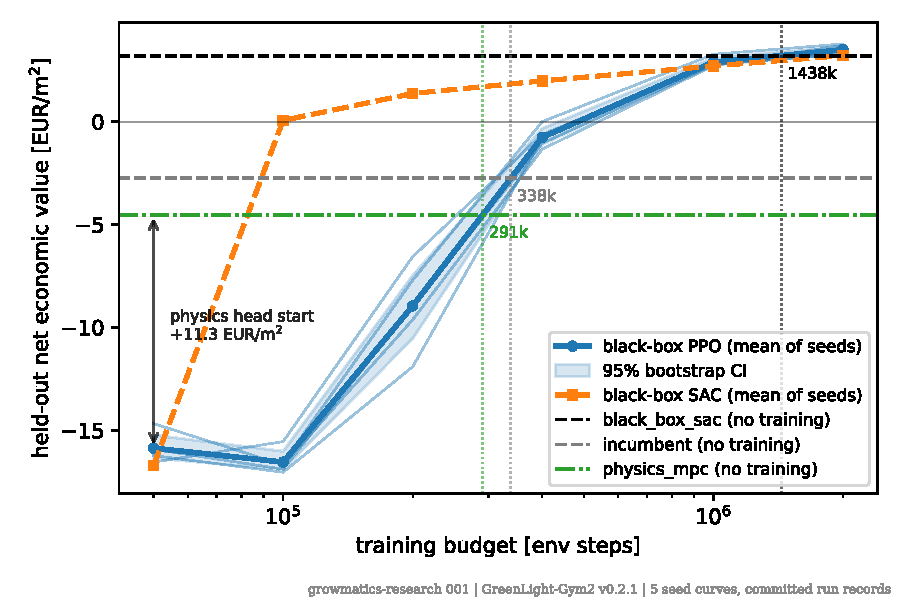
\includegraphics[width=0.9\linewidth]{fig-data-efficiency.pdf}
  \caption{Held-out net economic value against training budget (five seeds, mean with 95\% bootstrap CI). Horizontal lines mark the zero-training baselines; vertical markers give the measured crossover budgets, and the arrow the zero-training head start.}
  \label{fig:dataeff}
\end{figure}

\begin{table}[t]
  \centering\small
  \caption{Held-out net economic value [EUR\,m$^{-2}$] by training budget (5 seeds). Reproduce: \texttt{examples/analyze.py}.}
  \label{tab:dataeff}
  \begin{tabular}{rrrr}
    \toprule
    budget & mean & sd & 95\% CI \\
    \midrule
    50k  & $-15.86$ & $0.71$ & $[-16.35, -15.23]$ \\
    100k & $-16.54$ & $0.59$ & $[-16.91, -16.02]$ \\
    200k & $-8.95$  & $2.03$ & $[-10.54, -7.47]$ \\
    400k & $-0.76$  & $0.50$ & $[-1.11, -0.33]$ \\
    1M   & $+2.90$  & $0.23$ & $[+2.76, +3.11]$ \\
    2M   & $+3.50$  & $0.24$ & $[+3.32, +3.69]$ \\
    \bottomrule
  \end{tabular}
\end{table}

\subsection{The head-to-head comparison}

Table~\ref{tab:arms} gives the five-arm comparison at zero mismatch (the R1 anchor run); the mismatch axis, which decays the physics arms, is the following subsection.

\begin{table}[t]
  \centering\small
  \caption{Five-arm comparison at zero mismatch (R1 anchor, 84 seasons); the mismatch ladder decays the physics arms (following subsection), so this is the clean no-mismatch ranking.
  The $\pm$ values are across-season standard deviations, dominated by between-year
  weather difficulty; they are not the seed-level spread of the mean, which for the
  PPO arm is $0.24$ over five seeds (Table~\ref{tab:dataeff}).}
  \label{tab:arms}
  \begin{tabular}{lrrrrr}
    \toprule
    arm & net [EUR\,m$^{-2}$] & $n$ & gate(RH) & online [ms] & solve-succ. \\
    \midrule
    RL-in-MPC (physics-informed) & $+3.58 \pm 1.94$ & 20 & fail & 275.2 & 0.998 \\
    black-box PPO (2M)   & $+3.50 \pm 1.92$ & 20 & fail & 1.4 & -- \\
    black-box SAC (2M)   & $+3.21 \pm 1.93$ & 20 & fail & 0.4 & -- \\
    rule-based incumbent & $-2.74 \pm 5.41$ & 4$^{\ddagger}$  & fail & 0.1 & -- \\
    physics-only NMPC    & $-3.06 \pm 0.90$ & 20 & fail & 251.0 & 0.999 \\
    \bottomrule
  \end{tabular}

  \smallskip
  {\footnotesize $^{\ddagger}$the rule-based arm is GreenLight-Gym2's shipped setpoint controller with its default schedule, run without site-specific humidity tuning; it is a reference point, not a tuned commercial climate-computer strategy, and returns a net loss over this early-season window. It is deterministic, so its independent trials are the four weather years and its gate row is underpowered. The physics-only NMPC is likewise deterministic at zero mismatch (the perturbation draw vanishes), so its five seeds coincide and its independent trials here are also the four weather years; its genuine seed variation appears only at $m > 0$ (Table~\ref{tab:peryear-mismatch}). Online cost is wall-clock under uniform 20-worker load, hardware-stamped; valid as a relative axis.}
\end{table}

\begin{figure}[t]
  \centering
  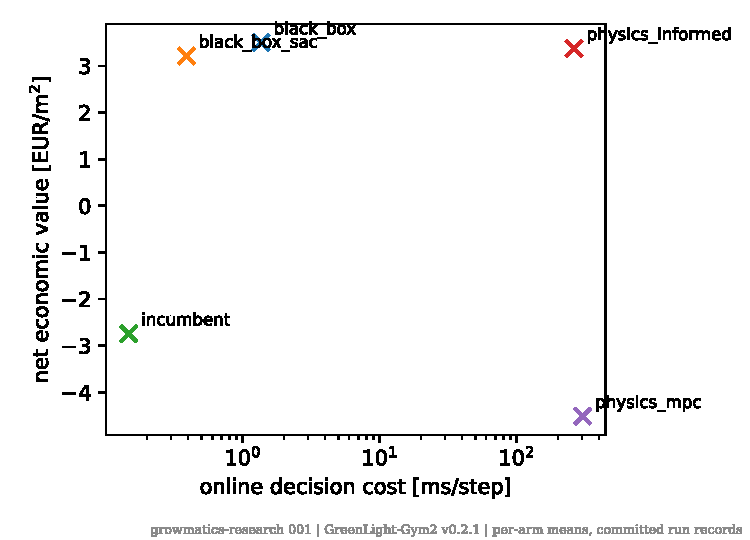
\includegraphics[width=0.7\linewidth]{fig-pareto.pdf}
  \caption{Net economic value against online decision cost (log scale), all five
  arms on the shared grid; up and to the left is better. Black-box PPO sits at the
  knee, attaining essentially the hybrid's net value at about 1/200 of its online
  cost. The physics-only NMPC is dominated (lower value and higher cost than PPO);
  the rule-based incumbent is cheapest but loss-making. All five arms fail the
  humidity gate under the native objective (crosses), so the trade-off is reported
  over all arms rather than a gate-passing subset; the anti-ideal reference point
  for the ranking is the worst observed value on each axis (net
  $-3.06$~EUR\,m$^{-2}$, cost $275.2$~ms).}
  \label{fig:pareto}
\end{figure}

Three findings stand, each backed by the paired analysis (Table~\ref{tab:stats}).
First, the hybrid wins: RL-in-MPC attains the best net value and beats its own guide
policy at matched conditions, a small but perfectly consistent margin (median
$+0.075$~EUR\,m$^{-2}$, $95\%$ CI $[+0.067, +0.085]$, winning all $20$ zero-mismatch
conditions, Cliff's $\delta = 1.0$, Wilcoxon $p = 1.9\times10^{-6}$ raw, $9.5\times10^{-6}$ Holm-corrected;
Figure~\ref{fig:slope}). Both learned arms dominate the physics-only NMPC by roughly
$7$~EUR\,m$^{-2}$ (Holm-corrected $p < 10^{-5}$). The mean gap over PPO is tiny
because between-year weather difficulty dominates the marginal spread; pairing removes it
and exposes the consistent advantage. Second, the myopic economic NMPC does not beat the deployed rule-based incumbent on net value, echoing the horizon limitation reported by the testbed's authors \citep{vanlaatum2026rlmpc} and the classical two-time-scale analysis of greenhouse optimal control, where the slow crop dynamics carry the economics a 1-hour horizon cannot see \citep{vanhenten2009timescale}. Economic MPC theory addresses this through terminal ingredients, a terminal cost or dissipativity-based design that restores approximate infinite-horizon optimality under a short horizon \citep{angeli2012economicmpc, mayne2014mpcpromise}; our formulation carries none of these (soft penalties, no terminal set), so the myopic result is a property of this deliberately minimal economic NMPC and not of physics-based control in general, since arm 4 already supplies the terminal cost-to-go a short horizon otherwise lacks (Section~\ref{sec:limitations}). Third, every arm violates the humidity bound in every season under the strict any-step
gate ($284/284$ across the full grid), confirming that a reward which prices violations invites trading them
for revenue and that feasibility must be gated rather than priced. The strict gate,
however, cannot rank the arms; the banded gate and degree-hours (Eq.~\ref{eq:gate},
Figure~\ref{fig:gate}) reveal a sharp separation the any-step flag hides
(Table~\ref{tab:gate}): the learned controllers breach the bound briefly and shallowly
(the learned controllers accumulate $72$--$131$ RH degree-hours per season --- SAC $72$, PPO $107$, RL-in-MPC $131$ --- and
banded-violate $60$--$80\%$ of seasons), while the physics-only MPC and the
rule-based incumbent sit in gross violation for most of the season ($983$ and $852$
degree-hours, $100\%$ banded). Humidity discipline, not just economic value, separates
the learned arms from the physics baselines.

\begin{table}[t]
  \centering\small
  \caption{Humidity gate at three resolutions, zero mismatch (R1 anchor). The strict gate
  saturates; the banded gate and degree-hours discriminate.}
  \label{tab:gate}
  \begin{tabular}{lrrr}
    \toprule
    arm & strict (any step) & banded ($>$2 pt, $>$1 h) & RH degree-hours \\
    \midrule
    black-box PPO   & 20/20 & 16/20 & 107 \\
    black-box SAC   & 20/20 & 12/20 & 72 \\
    RL-in-MPC       & 20/20 & 16/20 & 131 \\
    physics-only NMPC & 20/20 & 20/20 & 983 \\
    rule-based incumbent & 4/4 & 4/4 & 852 \\
    \bottomrule
  \end{tabular}
\end{table}

\begin{figure}[t]
  \centering
  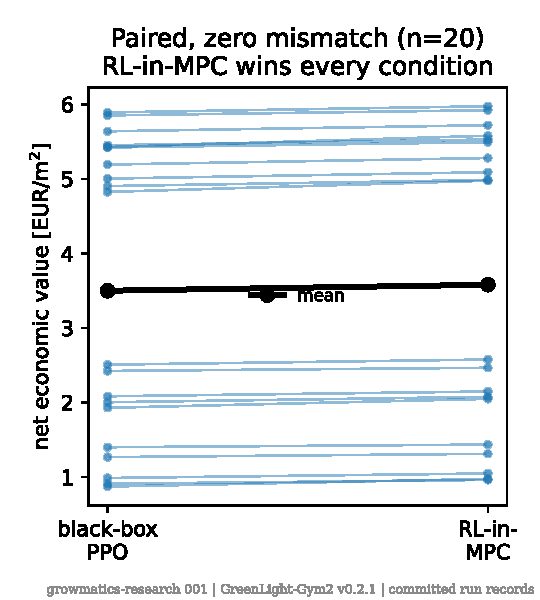
\includegraphics[width=0.42\linewidth]{fig-paired-slopegraph.pdf}
  \caption{Paired net value at zero mismatch: one line per matched (weather-year, seed)
  condition ($n = 20$). RL-in-MPC exceeds its black-box guide policy on every condition
  (Cliff's $\delta = 1.0$), a consistency invisible in the near-equal marginal means.}
  \label{fig:slope}
\end{figure}

\paragraph{Year variation and leave-one-year-out robustness.} Absolute net value swings widely across the four held-out weather years \emph{at zero mismatch} (Table~\ref{tab:peryear}; we compare all five arms at $m=0$ because that is the only ladder level at which every arm is defined --- the mismatch axis perturbs the physics arms only, Section~\ref{sec:results} below). The deployed incumbent ranges from $+2.04$ (2022) to $-9.44$~EUR\,m$^{-2}$ (2023), a $12.5$ spread, because a fixed rule-based schedule is fragile to weather difficulty. Every arm ranks the years the same way (2023 hardest, 2022 and 2025 easiest), so the spread is weather, not controller. Two structural readings follow. First, the myopic NMPC is the \emph{most} year-stable arm (spread $2.3$) precisely because it acts least, and the incumbent-versus-NMPC ordering flips with year difficulty: the incumbent wins in easy years, the NMPC in hard ones. Second, despite the swing the arm ranking is invariant \emph{within} every year and the paired advantages are preserved, which is why the analysis pairs on (year, seed) rather than pooling raw seasons. A leave-one-year-out check confirms no single year drives the result: dropping each year in turn moves PPO's held-out mean within $[+2.78, +4.30]$~EUR\,m$^{-2}$ (dropping the hard 2023 raises it, the easy 2025 lowers it), while the arm ranking and the sign of every headline comparison are unchanged under all four drops. The per-year view also extends to the mismatch axis for the two model-based arms (Table~\ref{tab:peryear-mismatch}), and it shows the robustness is itself \emph{year-invariant}: out to $20\%$ mismatch the hybrid decays by at most $0.9$~EUR\,m$^{-2}$ in every year while the pure NMPC loses $3$ to $5$ in every year, so the physics-arm gap of $+9$ to $+11$~EUR\,m$^{-2}$ at $20\%$ mismatch holds \emph{within each weather year}, not merely on average. A weather-covariate regression that attributes the spread to season radiation and heating demand is deferred to the reproducibility appendix.

\begin{table}[t]
  \centering\small
  \caption{Held-out net economic value [EUR\,m$^{-2}$] by weather year, at zero mismatch (spread $=\max-\min$ across years). The learned and hybrid arms share the year ordering; the incumbent's $12.5$ spread quantifies rule-based fragility. Reproduce: \texttt{examples/peryear\_tables.py}.}
  \label{tab:peryear}
  \begin{tabular}{lrrrrrr}
    \toprule
    arm & 2022 & 2023 & 2024 & 2025 & mean & spread \\
    \midrule
    incumbent   & $+2.04$ & $-9.44$ & $-6.65$ & $+3.09$ & $-2.74$ & $12.5$ \\
    PPO         & $+5.08$ & $+1.09$ & $+2.19$ & $+5.65$ & $+3.50$ & $4.6$ \\
    SAC         & $+4.81$ & $+0.77$ & $+1.91$ & $+5.36$ & $+3.21$ & $4.6$ \\
    NMPC        & $-3.05$ & $-3.93$ & $-3.66$ & $-1.61$ & $-3.06$ & $2.3$ \\
    RL-in-MPC   & $+5.17$ & $+1.15$ & $+2.26$ & $+5.74$ & $+3.58$ & $4.6$ \\
    \bottomrule
  \end{tabular}
\end{table}

\begin{table}[t]
  \centering\small
  \caption{Robustness is year-invariant: net value [EUR\,m$^{-2}$] of the two model-based arms by weather year at three mismatch levels (the learned and rule-based arms have no mismatch axis, so they do not appear). The hybrid holds in every year; the NMPC degrades in every year. Reproduce: \texttt{examples/peryear\_tables.py}.}
  \label{tab:peryear-mismatch}
  \begin{tabular}{llrrrr}
    \toprule
    arm & $m$ & 2022 & 2023 & 2024 & 2025 \\
    \midrule
    \multirow{3}{*}{NMPC (physics-only)} & $0$    & $-3.05$ & $-3.93$ & $-3.66$ & $-1.61$ \\
                                         & $0.10$ & $-2.82$ & $-5.54$ & $-5.26$ & $-2.41$ \\
                                         & $0.20$ & $-6.77$ & $-8.51$ & $-8.80$ & $-5.98$ \\
    \midrule
    \multirow{3}{*}{RL-in-MPC (hybrid)}  & $0$    & $+5.17$ & $+1.15$ & $+2.26$ & $+5.74$ \\
                                         & $0.10$ & $+5.14$ & $+1.13$ & $+2.21$ & $+5.70$ \\
                                         & $0.20$ & $+4.59$ & $+0.38$ & $+1.60$ & $+4.84$ \\
    \bottomrule
  \end{tabular}
\end{table}

\subsection{Mismatch and reliability}

Figure~\ref{fig:mismatch} gives the advantage decay $\Delta(m) = \bar J_{\mathrm{arm}}(m) - \bar J_{\mathrm{arm}}(0)$, the benchmark's largest effect: across the $0 \to 20\%$ mismatch ladder the hybrid holds nearly flat ($+3.58 \to +2.85$, a $0.73$~EUR\,m$^{-2}$ decay) while pure NMPC decays steeply ($-3.06 \to -7.52$). Read against the deployed incumbent, both learned arms clear it by roughly $6$~EUR\,m$^{-2}$ (PPO $+6.24$; hybrid $+6.32$ at $m=0$, still $+5.59$ at $20\%$ mismatch), whereas the physics-only controller never clears the incumbent and falls further behind as mismatch grows ($-0.32 \to -4.78$); the physics-arm gap thus widens from $+6.6$ to $+10.4$~EUR\,m$^{-2}$. Because the mismatch axis perturbs only the parameters the model-based arm consumes, this quantifies the hybrid's insensitivity to model-based calibration error, not cross-class robustness; within that scope the effect is large and, on the six-level ladder, statistically significant: the arm-by-mismatch interaction (slope difference $-18.1$) has $p = 4.5\times10^{-13}$ in the mixed model $\text{net} \sim \text{arm} \times \text{mismatch} + (1\,|\,\text{year})$, so the learned guidance measurably insures the physics controller against its own model error, not merely as a directional effect. The insensitivity is year-invariant (Table~\ref{tab:peryear-mismatch}), not an averaging artifact. Solver reliability stays above the $0.9$ floor throughout (NMPC $0.999$, hybrid $0.995$).

The learned policies show no generalization gap: the five 2M policies average $+3.29$ on the eight training years versus $+3.50$ held-out (the difference is within year-difficulty variance), so the held-out plateau reflects genuine control skill rather than weather memorization.

\begin{figure}[t]
  \centering
  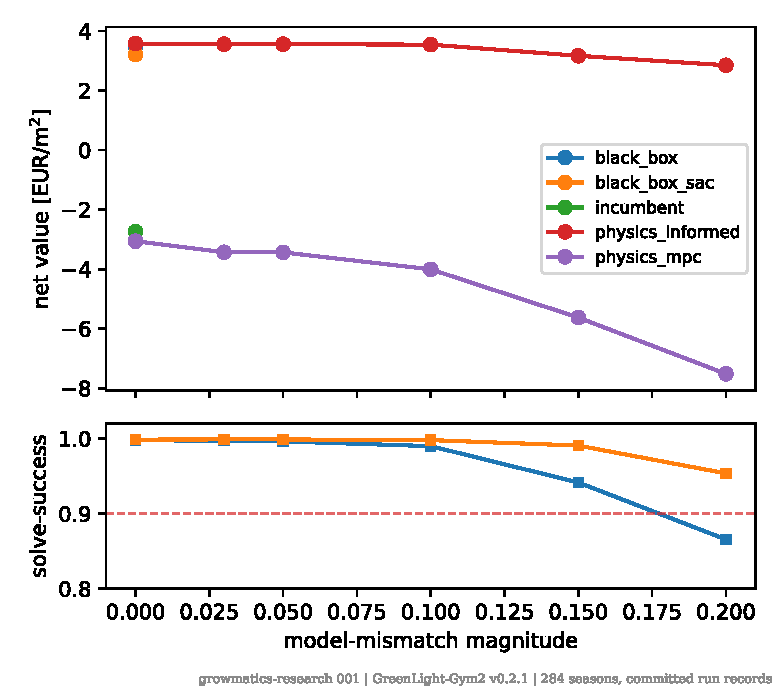
\includegraphics[width=0.85\linewidth]{fig-mismatch.pdf}
  \caption{Net value (top) and solver reliability (bottom) against controller-model mismatch. The hybrid's advantage survives model error; the pure-physics arm's does not.}
  \label{fig:mismatch}
\end{figure}

\begin{figure}[t]
  \centering
  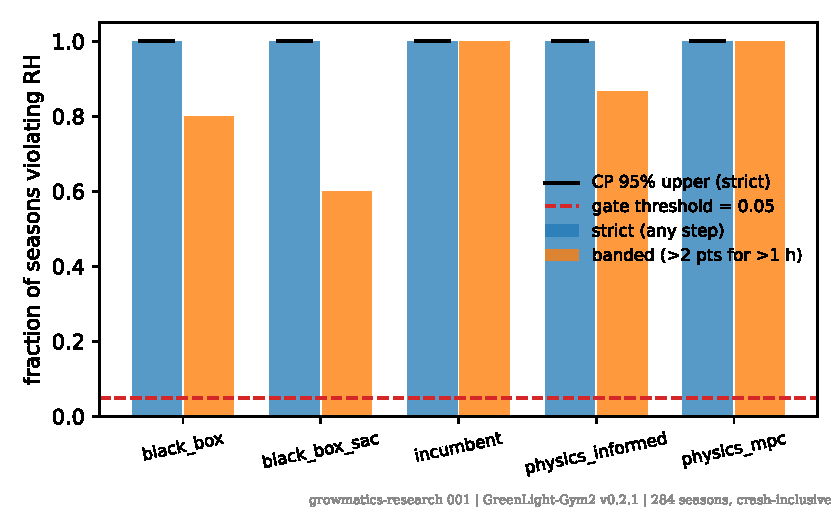
\includegraphics[width=0.8\linewidth]{fig-gate.pdf}
  \caption{Violating-season rates against the pre-registered $\varepsilon = 5\%$ gate (crash-inclusive Clopper--Pearson uppers). The native economic objective saturates the gate for every arm.}
  \label{fig:gate}
\end{figure}

\begin{table}[t]
  \centering\small
  \caption{Paired arm-versus-arm net value (Wilcoxon signed-rank, matched conditions,
  Holm-corrected). $n$ is matched (year $\times$ seed $[\times$ mismatch$]$) conditions;
  the deterministic incumbent's four conditions are underpowered ($p \ge 0.125$ is the
  floor at $n = 4$).}
  \label{tab:stats}
  \begin{tabular}{llrrrr}
    \toprule
    A & B & $n$ & median diff & Cliff's $\delta$ & $p$ (Holm) \\
    \midrule
    RL-in-MPC & black-box PPO & 20 & $+0.08$ & $1.0$ & $9.5\times10^{-6}$ \\
    RL-in-MPC & physics NMPC  & 120 & $+7.91$ & $1.0$ & $1.2\times10^{-20}$ \\
    RL-in-MPC & incumbent     & 4  & $+6.30$ & $1.0$ & $0.375$ \\
    black-box PPO & physics NMPC & 20 & $+6.60$ & $1.0$ & $9.5\times10^{-6}$ \\
    black-box PPO & incumbent  & 4  & $+6.24$ & $1.0$ & $0.375$ \\
    physics NMPC & incumbent  & 4  & $-0.85$ & $0.0$ & $1.000$ \\
    \bottomrule
  \end{tabular}
\end{table}

\section{Discussion}\label{sec:discussion}

\paragraph{Data cost of matching physics.} The crossover budgets ($\approx$317k steps against NMPC, $\approx$338k against the incumbent; log-budget interpolation of the mean curve, derivation in the benchmark record) translate to roughly 55 simulated growing seasons of interaction: an amount of experience no commercial greenhouse can supply. In simulation the learned policy wins outright; on a real greenhouse the physics head start ($+12.8$~EUR\,m$^{-2}$ of the pure NMPC over the least-trained, $50$k-step policy, a lower bound on its lead over a fully untrained one) is the operative fact, since 55 seasons of interaction is unavailable. The hybrid does not escape this: it requires the fully trained 2M-step guide policy, so it inherits the training cost rather than banking the head start. The honest deployment reading is that black-box RL is the pragmatic simulator winner, physics-only control is the zero-data option, and the hybrid is worth its two-orders-of-magnitude online cost only where insensitivity to parametric model error is worth more than compute, a case this testbed does not settle.

\paragraph{The hybrid's measured advantage.} On the paper's own Pareto axes, black-box PPO is the controller to deploy: at matched conditions it equals the hybrid's net value ($+3.50$ vs $+3.58$), at about $1/200$ of its online cost ($1.4$ vs $275.2$~ms per step) and with fewer humidity degree-hours ($107$ vs $131$). The hybrid is therefore not Pareto-dominant over its own guide policy. Its one measured advantage is insensitivity to parametric model error, and the mechanism is not that ``physics contributes robustness'': the mismatch axis perturbs only the nominal parameters the \emph{model-based} arm consumes, while the model-free guide (selected on roughly $93\%$ ($89$--$96\%$ across the ladder) of steps) ignores them by construction, so the hybrid is flat under mismatch because its dominant component cannot see the perturbed model.
A control-meaningful robustness test would perturb a quantity both arms are exposed to, such as weather-forecast (preview) error, which the greenhouse optimal-control literature treats as the operative uncertainty \citep{vanhenten2009timescale} and which both controller classes here consume; the present parametric axis is a bound on structured model-based calibration error only, not a cross-class robustness comparison, and drawing each parameter independently further understates it since real calibration error is structured and correlated. A shared-exposure forecast-error axis is the natural next test and is left to follow-on work.

\paragraph{Gate calibration as a finding.} As pre-registered ($\varepsilon = 5\%$, any-step violation), the gate saturates: every season of every arm violates. We report this rather than tune it away; it quantifies how far the field's standard economic objective sits from grower-trustable humidity discipline. Alongside it we report a pre-specified banded variant (violation only if RH exceeds the
bound by more than 2 points for more than one consecutive hour, grounded in the reference
MPC's own margin) and per-season degree-hours. Together they turn a saturated column into
a finding: the strict gate shows nobody is clean, but degree-hours show that the learned
controllers fail \emph{gently} (roughly $70$--$130$ RH degree-hours) while the
physics-only MPC and the incumbent fail \emph{grossly} (over $830$), roughly an order-of-magnitude
difference. Humidity safety, measured continuously, is a second axis on which physics
alone underperforms the learned and hybrid controllers on this testbed.

\paragraph{The general structure: short-horizon planning plus a learned long-horizon value.} The mechanism this benchmark isolates is not particular to greenhouses or to MPC. A short-horizon economic controller is myopic because the payoff lies beyond its horizon; supplying a \emph{learned long-horizon value} restores far-sighted behaviour. This is the same structure that recurs across sequential decision-making: a shallow tree search made strong by a learned value network at its leaves in board games \citep{silver2016alphago}, a short-horizon model-predictive controller made strong by a learned terminal value in robotics \citep{hansen2022tdmpc, lowrey2019polo}, and, unifying both, the approximate-dynamic-programming view of predictive control as rollout with a terminal cost-to-go approximation \citep{bertsekas2019rloptimalcontrol}. Our arm~4 is the greenhouse instance of that pattern, and the $-3.1$-to-$+3.6$~EUR\,m$^{-2}$ swing in mean net value from pure NMPC to the RL-in-MPC hybrid is a direct measurement of what the learned terminal value is worth.

\paragraph{Beyond greenhouses.} The trade this benchmark isolates is not specific to greenhouses. Any economically-driven controller on a constrained physical system, deployed under a model it does not perfectly trust, faces the same three-way choice between training-free physics, data-hungry learning, and a hybrid whose value rests on parametric-error insensitivity. Building climate control and distributed-energy-resource scheduling (heat pumps, batteries, and storage operated against a time-varying tariff) share the greenhouse's structure: a slow storage state, a hard operating limit, and an energy-dominated objective, a domain where learned control has already been reported to outperform a rule-based baseline on a heat-pump storage system \citep{jang2026offlinerlgreenhouse}. What we argue transfers is the measurement rather than the numbers: solver reliability and a hard feasibility gate belong alongside economic value as first-class deployment axes on any such system, while the crossover budget and the size of the physics head start are testbed-specific and must be re-measured per domain.

\section{Limitations}\label{sec:limitations}

Single simulator and crop; deterministic plant (within-platform bit-reproducibility, floating-point tolerance across platforms); wall-clock online cost is hardware- and load-stamped, valid relatively; the incumbent contributes only four independent seasons on the deterministic plant (its gate row is flagged underpowered); mismatch is parametric perturbation of the nominal model, an upper bound on the structured-error story real greenhouses present, since a parametric perturbation preserves the model's functional form and is invisible to the model-free arms. Further limitations a domain or control reader will note: the rule-based reference is untuned and loss-making over this window (it anchors the Pareto reference, so ``improvement over the incumbent'' should be read against a reference, not a competitive baseline); the humidity metric (degree-hours above the bound) is not disease-grounded and does not separate a benign daytime excursion from a dangerous night-time near-saturation; the black-box corner is represented by PPO and, after equal-procedure random-search tuning, SAC (2M five-seed held-out net $+3.21$, positive by ${\sim}100$k steps with no mid-training valley, versus PPO's $+3.50$); both learned arms make the data-efficiency claim, so it is not a PPO artifact, though RecurrentPPO and other classes remain untested. The safety profile is analysed for the humidity class only: the run records also hold the temperature, CO$_2$, and lamp classes, and under the temperature band the physics-only NMPC accumulates roughly ten times the degree-hours of every other arm while the three learned arms, unlike the incumbent, exceed the band for over an hour in every season, a profile this paper leaves unanalysed.

\section*{Acknowledgments}

This work was funded by Growmatics B.V. as part of its internal research program. The author thanks colleagues at Growmatics and Breda University of Applied Sciences for helpful discussions, and the authors of GreenLight-Gym2 and of the GreenLight model for releasing their simulators openly; weather data are from the Open-Meteo archive.

\section*{Reproducibility statement}

Every number in this paper traces to a committed JSON run record (git commit, hardware stamp, grid, failures) in the released repository; the analysis pipeline regenerates all tables and figures from those records with one command. The plant is bit-deterministic within a platform (verified $\Delta = 0$ on repeat runs of every arm), and the NMPC seasons reproduce exactly only with the math libraries pinned to one thread (\texttt{OMP\_NUM\_THREADS=1}, as in the recorded run): under default threading the IPOPT path diverges over the 5760 solves and a season's net value shifts by about $0.1$~EUR\,m$^{-2}$; PPO training follows the testbed's published recipe read from its pinned source. The
source data underlying every figure and statistical test is the committed per-season run
record; a per-artifact command map (which script and input file regenerates each table and figure) is in \texttt{manuscript/REPRODUCE.md}, and the anchor is \texttt{benchmark\_r1-union.json}. The tables and figures regenerate via \texttt{examples/analyze.py} and
all significance tests via \texttt{examples/stats.py}. The substrate is GreenLight-Gym2 v0.2.1 (commit \texttt{8bb5b28}); the controllers use CasADi 3.6.7 (which bundles IPOPT and the SUNDIALS/CVODES integrator), Stable-Baselines3 2.1.0 with sb3-contrib 2.1.0, Gymnasium 0.29.1, PyTorch 2.13.0, and NumPy 1.26.4.

\section*{Data and code availability}

The benchmark code for all five arms, the controller implementations, the committed run records, and the analysis pipeline that regenerates every reported table and figure will be released as a frozen open-source repository at \url{https://github.com/growmatics/greenhouse-control-benchmark} (release v1.0.0). The maintained successor of that code, Phytotron \citep{phytotron2026}, is public (version 0.1.0, AGPL-3.0-or-later) and reproduces this study's rule-based incumbent on all four held-out years and its physics-only NMPC season to six decimals, as its validation page documents; it ships no trained policy and no RL-in-MPC arm, and it gates seasons with crop-literature rules fixed after this study's run, so the frozen repository remains the reference for the learned and hybrid arms and for the pre-registered gate. All inputs are public: weather data from Open-Meteo and the open GreenLight-Gym2 simulator (v0.2.1, pinned); no commercial-grower or otherwise proprietary data is used.

\bibliographystyle{unsrtnat}
\bibliography{references}

\end{document}